% SCIENCE Visual Guide 2.0.1 + AI_SKILLS_R5; Akulin--Karlov batch v2.
% Graph traces are visibly heavier than axes. All labels use anchored positions.
\documentclass[border=5pt]{standalone}
\usepackage{fontspec,unicode-math}
\setmainfont{Noto Sans}
\setsansfont{Noto Sans}
\setmathfont{STIXTwoMath-Regular.otf}
\usepackage{tikz}
\usetikzlibrary{arrows.meta,calc,patterns,decorations.pathreplacing,intersections}
\definecolor{ScienceInk}{HTML}{000000}
\definecolor{ScienceCurve}{HTML}{000000}
\definecolor{ScienceAux}{HTML}{000000}
\definecolor{ScienceMuted}{HTML}{000000}
\tikzset{
  axis/.style={draw=ScienceInk,line width=0.75pt,-{Latex[length=2.2mm,width=1.35mm]}},
  axisplain/.style={draw=ScienceInk,line width=0.70pt},
  curve/.style={draw=ScienceCurve,line width=2.15pt,line cap=round,line join=round},
  curveb/.style={draw=ScienceAux,line width=1.95pt,dash pattern=on 6pt off 2.4pt,line cap=round,line join=round},
  curvedash/.style={draw=ScienceAux,line width=1.9pt,dash pattern=on 4pt off 3pt},
  optbeam/.style={draw=ScienceCurve,line width=1.75pt,-{Latex[length=2.2mm,width=1.3mm]}},
  optback/.style={draw=ScienceAux,line width=1.65pt,-{Latex[length=2mm,width=1.2mm]}},
  opt/.style={draw=ScienceInk,line width=1.0pt},
  opticplate/.style={draw=ScienceInk,line width=1.02pt,pattern=north east lines,pattern color=ScienceMuted},
  tick/.style={draw=ScienceInk,line width=0.7pt},
  textlabel/.style={text=ScienceInk,font=\fontsize{15}{18}\selectfont},
  smalllabel/.style={text=ScienceInk,font=\fontsize{13.5}{16.2}\selectfont},
}
\begin{document}
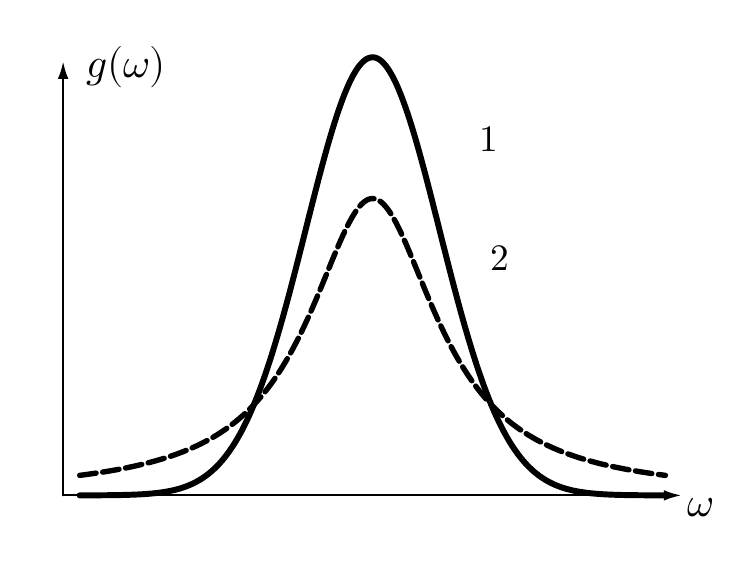
\begin{tikzpicture}[x=1cm,y=1cm,>=Latex,line cap=round,line join=round,font=\fontsize{15}{18}\selectfont]


% Compact aspect ratio, equal FWHM=2d, equal integrals.
% A_G/A_L = sqrt(pi*ln 2); curve 1 Gaussian, curve 2 Lorentzian.
\path[use as bounding box] (0,0) rectangle (8.7,6.6);
\draw[axis] (.45,.66)--(8.30,.66);
\draw[axis] (.45,.66)--(.45,6.17);
\node[textlabel,anchor=west] at (.62,6.10) {$g(\omega)$};
\node[textlabel,anchor=west] at (8.26,.51) {$\omega$};
\pgfmathsetmacro\AG{sqrt(pi*ln(2))}
\draw[curve,samples=410,domain=-3.72:3.72,smooth] plot ({4.38+1.0*\x},{.66+3.77*\AG*exp(-ln(2)*(\x)^2)});
\draw[curveb,samples=410,domain=-3.72:3.72,smooth] plot ({4.38+1.0*\x},{.66+3.77/(1+(\x)^2)});
\node[smalllabel,anchor=west,fill=white,text=ScienceCurve,inner sep=2pt] at (5.66,5.18) {$1$};
\node[smalllabel,anchor=west,fill=white,text=ScienceAux,inner sep=2pt] at (5.80,3.67) {$2$};

\end{tikzpicture}
\end{document}
